%!TEX TS-program = xelatex
\documentclass[]{friggeri-cv}
\usepackage{afterpage}
\usepackage{hyperref}
\usepackage{color}
\usepackage{xcolor}
\usepackage{fontspec}
\usepackage[utf8]{inputenc}

\hypersetup{
    pdftitle={Wesley Banfield CV},
    pdfauthor={Wesley Banfield},
    pdfsubject={CV},
    pdfkeywords={CV Wesley Banfield},
    colorlinks=false,
    allbordercolors=white
}

\RequirePackage{xcolor}
\definecolor{pblue}{HTML}{0395DE}

\begin{document}

\begin{figure}[!h]
	\begin{minipage}{0.48\textwidth}
		\begin{flushleft}
			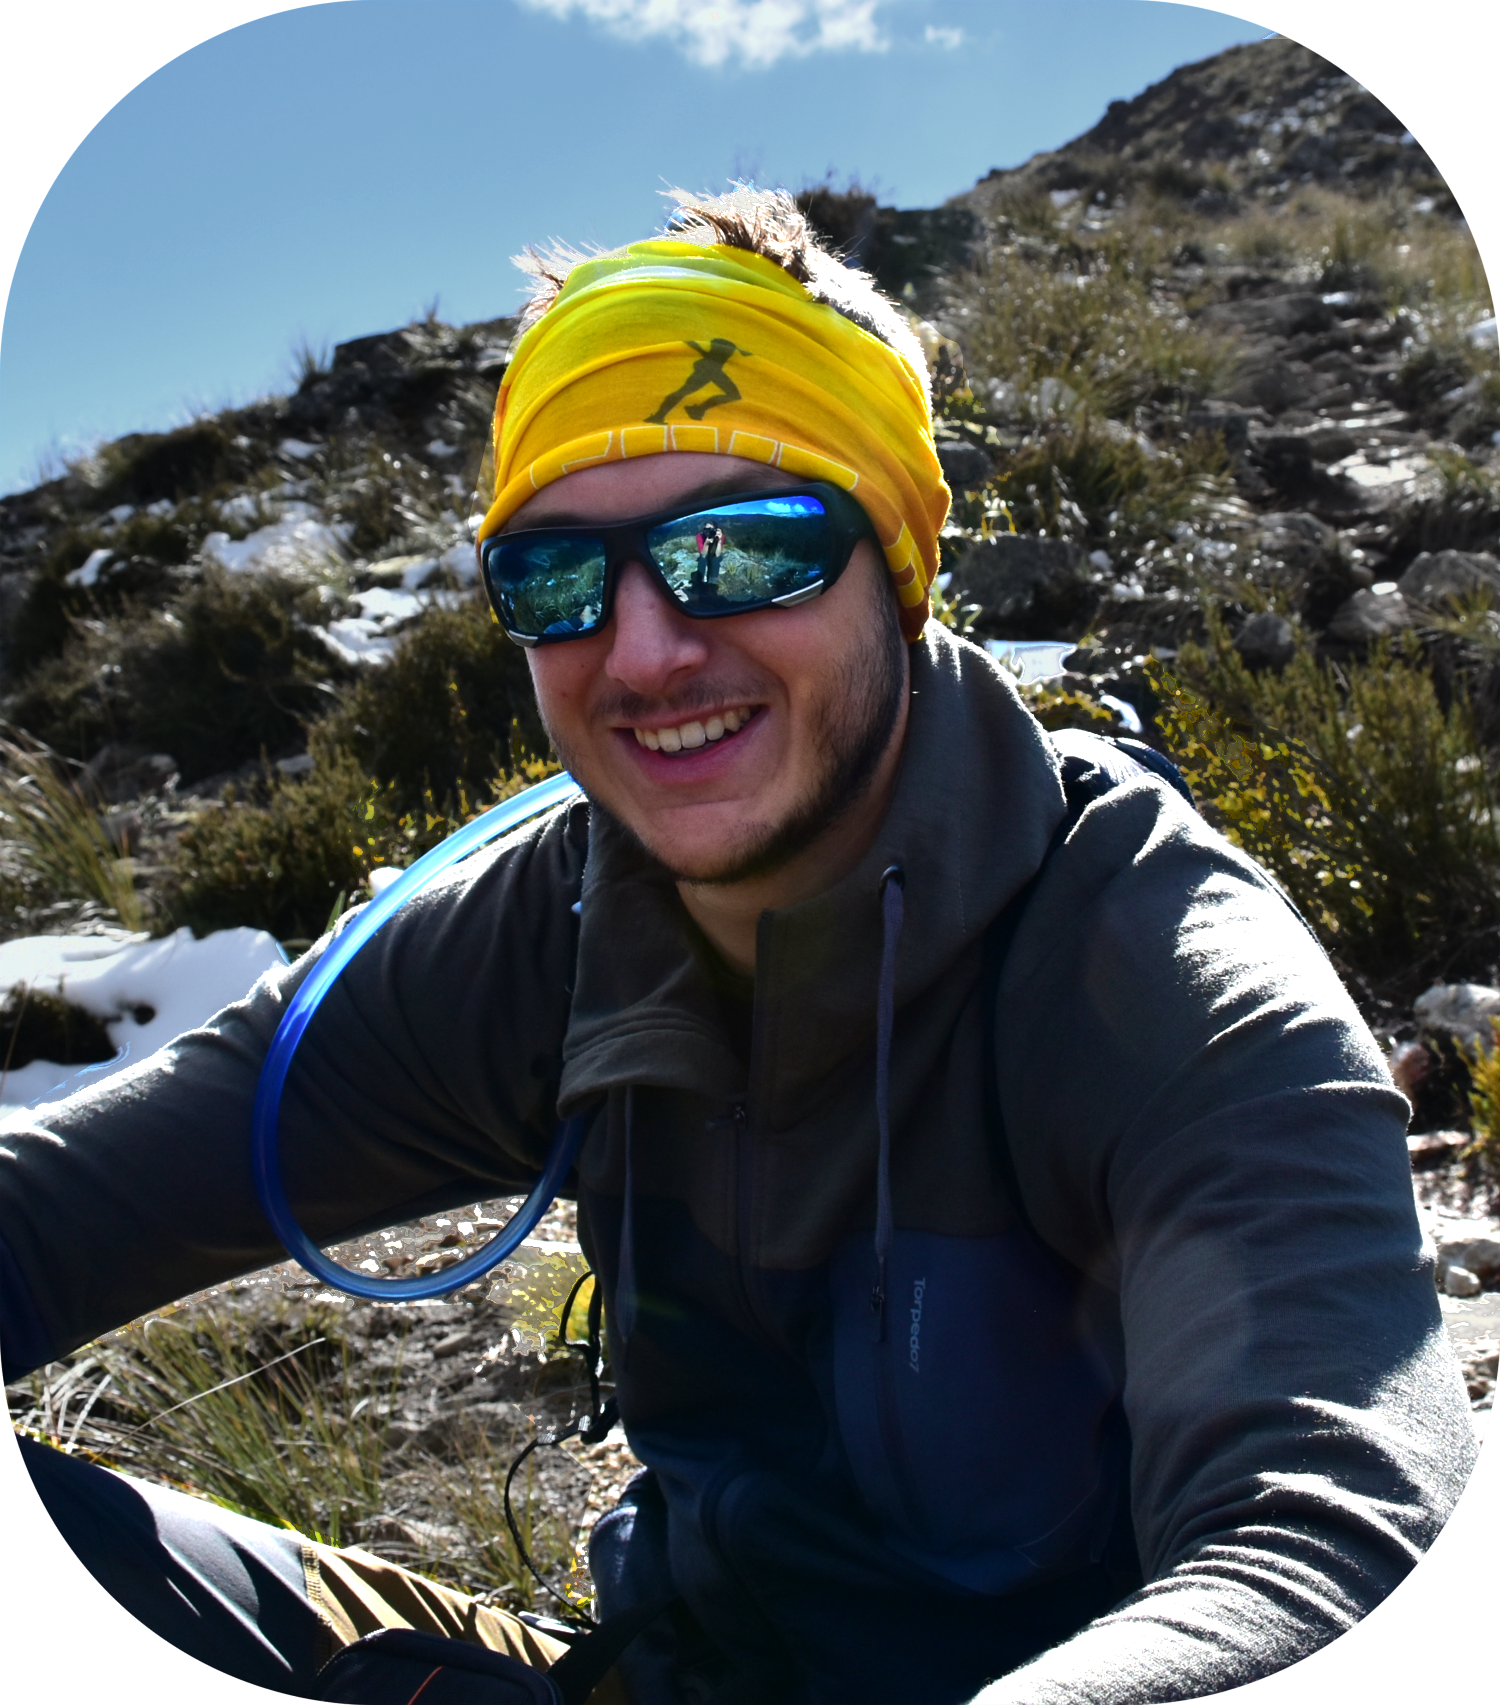
\includegraphics[width=2.75cm]{img/profile_relaxed.png}
		\end{flushleft}
	\end{minipage}\hfill
	\header{Wesley}{ Banfield}
 	{Full Stack Developer - Geoscientist}
	\begin{minipage}{0.48\textwidth}
		\begin{flushright}
			
\includegraphics[width=2.75cm]{img/qrcode.png}
		\end{flushright}
	\end{minipage}
\end{figure}
\vspace{-0.75cm}
% Fake text to add separator      
\fcolorbox{white}{gray}{\parbox{\dimexpr\textwidth-2\fboxsep-2\fboxrule}{%
.....
}}

\begin{quote}
\large
\begin{center}
Innovative engineer looking to \textbf{unite cutting edge web technologies and geosciences} to help provide a more sustainable future.
\\
\end{center}
\end{quote}

\begin{center}
\vspace{6pt}
\href{mailto:wesleybanfield@gmail.com}{\textbf{wesleybanfield@gmail.com}}
\\+33 7 52 08 02 37, Albertville, France
\\\emph{GB / USA citizen, FR bilingual}
\vspace{3pt}
\\\href{https://www.linkedin.com/in/wesleybanfield/}{LinkedIn},
\href{https://github.com/WesleyTheGeolien}{GitHub}
\href{https://wesleythegeolien.github.io}{website}
\end{center}

% \vspace{6pt}
\section{Domains of expertise}
\begin{itemize} 
	\item {\large\textbf{\textcolor{pblue}{Languages and Frameworks}}}: Python, Docker, TypeScript, React, Azure, C++, SQL, Latex
	\item {\large\textbf{\textcolor{pblue}{Backend}}}: Containerization, APIs, Data access, Serverless Compute, Micro Services
	\item {\large\textbf{\textcolor{pblue}{Domains}}}: Scientific Code, Visualisation, Innovation, Prototyping
\end{itemize}

\vspace*{\fill}
\section{Experience}
\begin{entrylist}
	
	\entry
	{8/21 - Now}
	{Senior Full Stack Developer}
	{\href{https://resourcemodelingsolutions.com/}{Resource Modeling Solutions}}
	{
	\\[-0.5em]
	\textbf{Full Stack: }Developement of 3D interactive web viewer and data processing pipeline.
	\\[3pt]
	\textbf{Large Language Model: }Develop and deploy a RAG LLM api to assist rmsp users. 
	\\[3pt]
	\textbf{Integrations: }Integration of RMS's Drillhole Optimizer C library into rmsp. Intergration bewteen RMSP and GeologicAI.
	\\[3pt]
	\textbf{Software Engineering: }Developement and maintenance of the core advanced geostatistical code base.
	\\[3pt]
	\textbf{Frontend: }Developement of \href{https://resourcemodelingsolutions.com}{company's website}.
	}

	\entry
	{2023}
	{Team Lead Tech and Infrastructure (Volonteer)}
	{\href{https://sites.google.com/climatematch.io/academy/about}{Climatematch}}
	{
		\\[-0.5em]
		\textbf{DevOps: }Test and deploy the \href{https://comptools.climatematch.io/tutorials/intro.html}{jupyter book} of the course content. 
		\\[3pt]
		\textbf{Management: }Coordinate the tech team to ensure software engineering best practices.
		\\[3pt]
		\textbf{Infrastructure: }Point of contact with \href{https://2i2c.org}{2i2c} to deploy JupyterHub for course.
	}
  
	\entry
	{9/20 - 7/21}
	{Research Engineer - Climate}
	{\href{https://paleoclim-cnrs.github.io/}{Protisvalor - CEREGE}}
	{
	\\[-0.5em]
	\textbf{Full Stack: } Design and implement a SaaS app to setup the IPSL boundary limits. The project is open source on \href{https://cerege-cl.github.io/netcdf_editor_app/}{GitHub}
	\\[3pt]
	\textbf{Infrastructure: } Deploy and maintain and provision the work group's JupyterHub and compute environments.
	\\[3pt]
	\textbf{Frontend: } Design and implement \href{https://paleoclim-cnrs.github.io}{work group's website}.
	}
	
 	\entry
	{10/19 - 6/20}
	{Project Manager Digital Innovation}
	{\href{http://envisol.net/}{Envisol, France}}
	{
	\\[-0.5em]
	\textbf{Full Stack: } Build a prototype SaaS application for data acquisition and interpretation for the Contamination and Remediation industry.
	\\[3pt]
	\textbf{Automation: } GIS data collection and processing.
	}
  
 	\entry
    {01/17 - 05/19}
    {Research Engineer}
    {\href{https://www.seequent.com/}{Seequent, Christchurch New Zealand}}
    {
    \\[-0.5em]
   	\textbf{Prototyping: }Web based dashboard creation, integration of Jupyter into workflows and deploying compute intensive tasks to the cloud.
   	\\[3pt]
   	\textbf{Core IP Reusage: }Automated creation of geological models from sub sets of data to sample geological uncertainty.
    \\[3pt]
   	\textbf{Strategy: }Technical support for key business decisions including verification of geostatistical implementations and creation of infrastructure to obtain and analyse usage metrics of Leapfrog software. 
    \\[3pt]
	\textbf{Stakeholder Communication: }Client meetings, presentations and bespoke prototyping facilitated by mixed background.
    % \\
    % Reference : \href{mailto:tim.schurr@seequent.com}{Tim Schurr, Solutions Architect}
	}
  
	% \entry
    % {05/16 - 09/16}
    % {Software Integration Engineering Internship}
    % {\href{https://www.total.com/en}{Total, Pau France}}
    % {Discretization plays an important part in coupled Oil \& Gas basin modelling. Too fine, the computation time prevails, too coarse and the calculations do not converge. As a software integration engineer I implemented an interface with the \href{http://www.ring-team.org/software/ringmesh}{RINGMesh} library to dynamically re-mesh during simulations.\\ Reference : \href{mailto:tristan.cornu@total.com}{Tristan Cornu, Pore pressure and Rock Mechanics Specialist}}

    % \entry
    % {02/16 - 05/16}
    % {Research Intern}
    % {\href{http://www.ring-team.org/}{Ring Research Lab, Nancy France }}
    % {Research and implementation of different automatic simultaneous well log correlation algorithms and creation of a SKUA-Gocad plug-in. The master's thesis was carried out in the lab that originally developed SKUA-Gocad before commercialisation by Paradigm. The work was presented and published in the 2016 Ring Meeting. \\Reference : \href{mailto:Guillaume.Caumon@ensg.univ-lorraine.fr}{Dr. Guillaume Caumon, Head of Research team}}
    
	% \entry
    % {06/15 - 09/15}
    % {Software Engineering Internship}
    % {\href{https://www.seequent.com/}{Seequent, Christchurch New Zealand}}
    % {Design and development of a graphical user interface for geostatistical analysis in Leapfrog 3D Geological modelling suite, later integrated into Leapfrog EDGE. Implementation of different geostatistical algorithms.
    % \\
    % Reference : \href{mailto:tim.mclennan@seequent.com}{Tim McLennan}}

	% \entry
	% {09/14 - 05/15}
	% {Lab Research Project}
	% {\href{http://georessources.univ-lorraine.fr/}{GeoRessources, Nancy France}}
	% {Geochemistry can be used to date oil, however when in contact with water certain couples reset. The goal of the project was to develop an experimental protocol to analyse the behaviour of the Rhenium / Osmium couple. Automated graphing tools where developed to analyse the ICP-MS results.
	% 	\\
	% 	Reference : Raymond Michels}
\end{entrylist}
\newpage
\vspace*{\fill}
\section{Presentations and Publications}
\begin{entrylist}
	\entry
	{2021}
	{Reproducible Compute Environments with Docker}
	{Paleoclim France}
	{\href{https://wesleythegeolien.github.io/Presentations/docker_reproducible_envs/index.html}{Presentation to work group how container technology can be harnessed to produce reproducible coding environments for publications and work.}}
	\entry
	{2021}
	{Portable interactive Plotting with Javascript}
	{Software Underground}
	{1h30 talk on how to use Python with Javascript to create portable graphs that can be used in any web browser. Viewable on \href{https://www.youtube.com/watch?v=j\_4wkMzGvKs}{YouTube}}
	\entry
	{2020}
	{Prototyping for Geologists}
	{Transform 2020}
	{Short talk on building a infrastructure to rapidily build and deploy prototypes.
	Viewable on \href{https://youtu.be/rUbvueIF5f8?t=4130}{YouTube}.}
	\entry
	{2019}
	{JupyterLab Quick Start Guide}
	{Packt}
	{Coauthor of JupyterLab quick start guide.}
	\entry
	{2019}
	{Integration of BIM and the subsurface}
	{Indura Cluster}
	{Presentation demonstrating the integrations between Building Information Modeling and subsurface data.}
	\entry
	{2018}
	{How certain are you of your surfaces}
	{Seequent Lyceum Perth}
	{Presentation in front of over 200 mining experts on behalf of Seequent demonstarting the latest R\&D work carried out at the company. Viewable on \href{https://www.youtube.com/watch?v=jt26J5ljlA0}{YouTube}.}
	\entry
	{2016}
	{Current automatic well log correlation techniques}
	{Ring Consortium}
	{Presentation in front off over 100 Oil and Gas experts demonstarting my Master's thesis on automated well log correlation techniques. The Master's thesis was also published in the Proceedings.}
\end{entrylist}
\section{Open Source Contributions}
\begin{entrylist}
	\entry
	{2021}
	{Seismic Footprint removal Hackathon}
	{Transform 2021}
	{Build a tool to design filters for seismic data in the frequency domain. After the hackathon a web based tool (panel) was built and deployed to AWS.}
	\entry
	{2020 - 2021}
	{Pangeo collaborator}
	{Pangeo}
	{Take part in weekly catchups to discuss and better understand the intersection between computing and climate sciences}
	\entry
	{2020 - 2021}
	{SOS Mediterranée website update}
	{CartONG}
	{Refresh of the website to show boat rescues in the mediterranean sea.}
	\entry
	{2020}
	{Well Correlation tool Hackathon}
	{Transform 2020}
	{Build a web tool (Dash / plotly) to load LAS files and visualise them.}
\end{entrylist}
\section{Education MEng, MSc}
\begin{entrylist}
  \entry
    {2013 - 2016}
    {Master in Geological Engineering with specialisation in software developement}
    {\href{http://ensg.univ-lorraine.fr/english/}{French National School of Geological Engineering}}
    {\emph{Ecole Nationale Superieure de Geologie} is a leading French engineering school specialising in geosciences and delivering an Engineering diploma combined with a Master from the University of Lorraine.\\ 
    % \\
    % \emph{Curriculum}: Numerical Geology\\ 
    % \emph{Natural Sciences}: Hyrdogeology, Structural Geology, Geomorphology, Geophysics\\
    % \emph{Engineering Sciences}: Applied Maths, Fluid Dynamics, Statistics, Partial Differential Equations\\
    % \emph{Software Sciences}:  Software Development, Interface Design, Computer Geometry, Visualisation and Parallelism, Mathematical concepts of geomodelling, Finite Elementss\\
    \\
    \emph{Title of Thesis}: ”Current automatic well log correlation techniques, their advantages and drawbacks”.
    % \emph{References}: Dr. Guillaume Caumon, Jonathan Edwards\\
	}
  	
	% \entry
    % {2011 - 2013}
    % {\href{https://en.wikipedia.org/wiki/Classe_preparatoire_aux_grandes_ecoles}{Classes Preparatoires aux Grandes Ecoles}}
    % {Lycee Pierre de Fermat, Toulouse France}
    % {2 years of intensive general scientific courses before national exams for entry to the French Grandes Ecoles, carried out at Pierre de Fermat, one of the top preparatory schools finishing in the top 10\% nationally.\\ 
    % \emph{Main subjects}: Mathematics, Physics, Chemistry, Biology and Geology, \\}

\end{entrylist}
\vspace*{\fill}
\end{document}


% }
%     \end{entrylist}
%     \vspace*{\fill}
%     \newpage
%     \vspace*{18pt}

% 	\begin{entrylist}
% 	\entry{}{}{}{